\documentclass[%
 reprint,
%superscriptaddress,
%groupedaddress,
%unsortedaddress,
%runinaddress,
%frontmatterverbose, 
%preprint,
%showpacs,preprintnumbers,
%nofootinbib,
%nobibnotes,
%bibnotes,
 amsmath,amssymb,
 aps,
%pra,
%prb,
%rmp,
%prstab,
%prstper,
%floatfix,
]{revtex4-1}

\usepackage{graphicx}% Include figure files
\usepackage{dcolumn}% Align table columns on decimal point
\usepackage{bm}% bold math
%\usepackage{hyperref}% add hypertext capabilities
%\usepackage[mathlines]{lineno}% Enable numbering of text and display math
%\linenumbers\relax % Commence numbering lines

%\usepackage[showframe,%Uncomment any one of the following lines to test 
%%scale=0.7, marginratio={1:1, 2:3}, ignoreall,% default settings
%%text={7in,10in},centering,
%%margin=1.5in,
%%total={6.5in,8.75in}, top=1.2in, left=0.9in, includefoot,
%%height=10in,a5paper,hmargin={3cm,0.8in},
%]{geometry}

\usepackage{cmap} % Поиск в PDF
\usepackage[T2A]{fontenc} % Кодировка
\usepackage[utf8]{inputenc} % Кодировка исходного текста
\usepackage[english, russian]{babel} % Локализация и переносы
\frenchspacing % Более тонкая настройка пробелов 
\usepackage{multirow}
\usepackage[warn]{mathtext}
\usepackage{amssymb}
\usepackage{ dsfont }

% Переопределение англоязычного начертания каппа, фи и эпсилон, 
% а также знаков сравнения
\renewcommand{\epsilon}{\ensuremath{\varepsilon}}
\renewcommand{\phi}{\ensuremath{\varphi}} 
\renewcommand{\kappa}{\ensuremath{\varkappa}}
\renewcommand{\le}{\ensuremath{\leslant}}
\renewcommand{\leq}{\ensuremath{\leqslant}}
\renewcommand{\ge}{\ensuremath{\geslant}}
\renewcommand{\geq}{\ensuremath{\geqslant}}
\renewcommand{\emptyset}{\ensuremath{\varnothing}}

\usepackage{textcomp} 
\usepackage{indentfirst} % Красная строка
\usepackage{amsmath} % Текст в формулах
\usepackage{graphicx} % Графика
\DeclareGraphicsExtensions{.pdf,.png,.jpg}
\usepackage{pgfplots}
\pgfplotsset{compat=1.13}

%\usepackage{times}

\begin{document}

\title{Спектральный анализ электрических сигналов}
\thanks{3.6.1}

\author{Иван Едигарьев,}
\affiliation{
 Московский Физико-Технический Институт\\
 Факультет Общей и Прикладной Физики, 526т\\
}
%\date{\today}

\begin{abstract}
Цель работы: 1) изучение спектрального состава периодических электрических сигналов.

В работе используются: анализатор спектра СК4-56, генератор прямоугольных импульсов Г5-54, генератор сигналов специальной формы Г6-34, осциллограф С1-76.\\

В работе изучается спектральный состав периодических электрических сигналов различной формы: последовательности прямоугольных
импульсов, последовательности цугов и амплитудно-модулированных гармонических колебаний. Спектры этих сигналов наблюдаются с помощью
промышленного анализатора спектра и сравниваются с рассчитанными теоретически.


\end{abstract}

\pacs{Valid PACS appear here}% PACS, the Physics and Astronomy
                             % Classification Scheme.
%\keywords{Suggested keywords}%Use showkeys class option if keyword
                              %display desired
\maketitle

%\tableofcontent

\section{\label{sec:level1}Принцип работы спектроанализатора.}

Для исследования спектров в работе используется гетеродинный анализатор спектра типа СК4-56. 
Принцип работы анализатора заключается в следующем: входные цепи 
анализатора последовательно преобразуют поступающие на его вход колебания с разными частотами в колебания вполне определённой промежуточной частоты; выходной прибор (в нашем случае это электроннолучевая трубка — ЭЛТ) воспроизводит амплитуду сигнала промежуточной частоты. Напряжение, пропорциональное частоте сигнала, который в данный момент преобразуется в сигнал промежуточной частоты, подаётся на вход $X$ ЭЛТ; напряжение, пропорциональное амплитуде исследуемой гармоники, поступает на вход $Y$. На экране анализатора возникает, таким образом, график, изображающий зависимость амплитуды гармоник от частоты, т.е. Фурье-спектр исследуемого сигнала. Для преобразования частоты колебаний, относящихся к исследуемому участку спектра, в сигнал промежуточной частоты служит нелинейный элемент (смеситель), на вход которого подаются исследуемый сигнал и сигнал со вспомогательного генератора колебаний регулируемой
частоты (с гетеродина). При нелинейном сложении этих колебаний на
выходе смесителя возникают сигналы суммарной и разностной частоты.

Для анализа используется только разностный сигнал. Смешение частот
исследуемого сигнала и частоты гетеродина лежит в основе большинства
современных радиоприёмных устройств — супергетеродинов.

Упрощённая структурная схема, поясняющая последовательный супергетеродинный метод спектрального анализа внешнего сигнала, изображена на рис.~1. Исследуемый сигнал $f(t)$ поступает на смеситель, на
который одновременно подаётся напряжение с гетеродина. Разностный
по частоте сигнал подаётся на фильтр, пропускающий очень узкую полосу частот, усиливается, детектируется, вновь усиливается и подводится
на вертикальный вход ЭЛТ.\\
\\
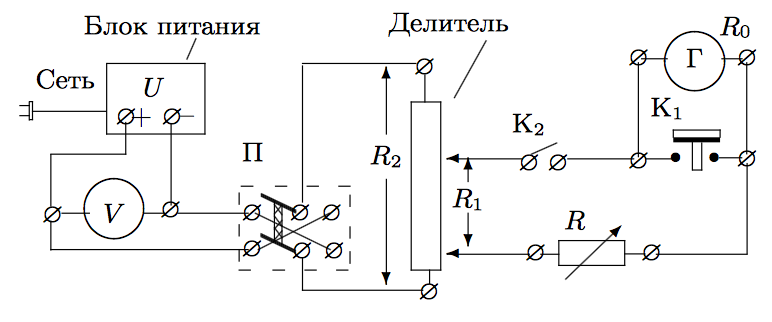
\includegraphics[scale = 0.27]{pic1.png}

Частота гетеродина управляется пилообразным напряжением, которое вырабатывается в генераторе развёртки. Сигнал с генератора подаётся также на горизонтальный вход ЭЛТ. Частота сигналов, вырабатываемых гетеродином, изменяется в пределах от $128$ до $188$ кГц. Фильтр
настроен на частоту $128$ кГц. Прибор анализирует, таким образом, колебания с частотами, лежащими между $128 - 128$ = $0$ кГц и $188 - 128 = 60$ кГц.

\section{\label{sec:level1}Исследование спектра периодической последовательности прямоугольных импульсов.}

\subsection{\label{sec:level2}Экспериментальная установка}

Схема для исследования спектра периодической последовательности прямоугольных импульсов представлена на рис. 2. Сигнал с выхода генератора прямоугольных импульсов Г5-54
подаётся на вход анализатора спектра и одновременно — на вход $Y$ осциллографа. С генератора импульсов на осциллограф подаётся также сигнал синхронизации, запускающий ждущую развёртку осциллографа. При
этом на экране осциллографа можно наблюдать саму последовательность
прямоугольных импульсов, а на экране ЭЛТ анализатора спектра — распределение амплитуд спектральных составляющих этой последовательности.\\
\\
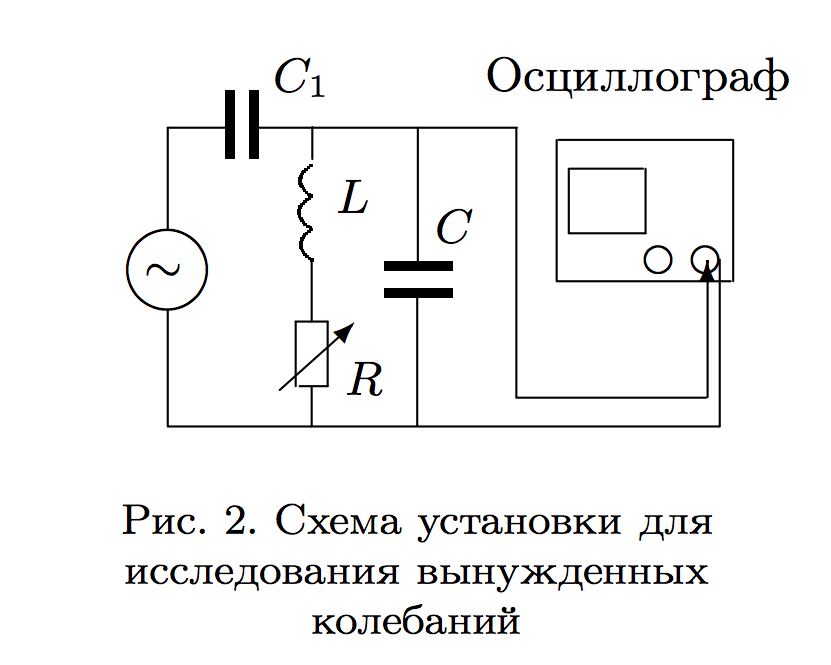
\includegraphics[scale = 0.27]{pic2.png}

В наблюдаемом спектре отсутствует информация об амплитуде нулевой гармоники, т. е. о величине постоянной составляющей; её местоположение (начало отсчёта шкалы частот) отмечено небольшим вертикальным выбросом.

\subsection{\label{sec:level2}Задание}

В этом упражнении исследуется зависимость ширины спектра периодической последовательности прямоугольных импульсов от длительности отдельного импульса.\\
1. Соберите схему согласно рис.~2 и включите в сеть только генератор Г5-54.\\
2. Познакомьтесь с назначением ручек управления генератора и осциллографа по техническому описанию, расположенному на установке (ТО,
разделы I и II).\\
3. Подготовьте установку к измерениям, следуя техническому описанию
(см. ТО, раздел III А).\\
4. Установив на анализаторе режим работы с однократной развёрткой, получите на его экране спектр импульсов с параметрами $f_{\text{повт}} = 10^3$~Гц;
$\tau$ = 25 мкс; частотный масштаб $m_x$ = 5 кГц$/$дел (см. ТО, III A, п. 7).\\
5. Проанализируйте, как меняется спектр ($\Delta{\nu}$ и $\delta{\nu}$ на рис. П.3): а) при
увеличении $\tau$ вдвое при неизменном $f_{\text{повт}}$ = 1 кГц; б) при увеличении
$f_{\text{повт}}$ вдвое при неизменном $\tau$ = 25 мкс. Опишите результаты или зарисуйте в тетрадь качественную картину.\\
6. Проведите измерения зависимости ширины спектра от длительности импульса $\Delta{\nu(\tau)}$ при увеличении $\tau$ от 25 до 200 мкс (6–8 значений при $f_{\text{повт}}$ = 1 кГц и масштабе по горизонтали $m_x$ = 5 кГц/дел).\\
7. Скопируйте на кальку огибающие спектров с параметрами: $f_{\text{повт}}$ = 1 кГц,
$m_x$ = 5 кГц/дел, а) $\tau$ = 50 мкс, б)$\tau$ = 100 мкс. Запишите на кальках эти
параметры и приложите кальки к отчёту.\\
8. Постройте график $\Delta{\nu(1/\tau)}$ и по его наклону убедитесь в справедливости
соотношения неопределённостей.

\section{\label{sec:level1}Исследование спектра
периодической последовательност
и цугов
гармонических
колебаний.}

\subsection{\label{sec:level2}Экспериментальная установка}

Исследование спектра периодически
чередующихся цугов гармонических
колебаний проводится по схеме,
изображённой на рис.~3.
Генератор Г6-34 вырабатывает синусоидальные
колебания высокой частоты. На вход АМ (амплитудная модуляция) генератора Г6-34 подаются прямоугольные импульсы с генератора Г5-54 и синусоида модулируется
— «нарезается» на отдельные куски — \textit{цуги}. Эти цуги с выхода генератора Г6-34 поступают на вход спектроанализатора и одновременно на вход $Y$ осциллографа. Сигнал синхронизации подаётся на вход $Х$ осциллографа с генератора импульсов.\\
\\
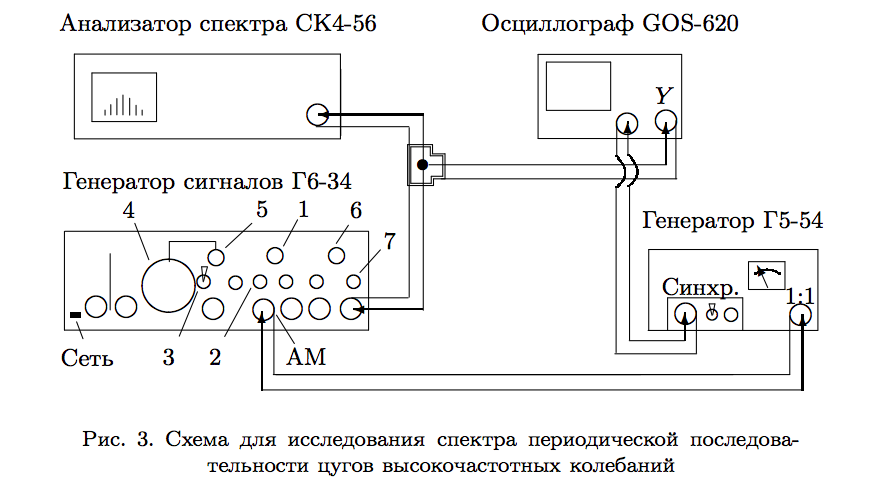
\includegraphics[scale = 0.27]{pic3.png}

\subsection{\label{sec:level2}Задание}

В этом упражнении исследуется зависимость расстояния между ближайшими спектральными
компонентами от частоты повторения цугов.\\
1. Соберите схему, изображённую на рис.~3.\\
2. Подготовьте приборы к работе, следуя техническому описанию (ТО, раздел III, Б).\\
3. Установив частоту несущей $\nu_0$ = 25 кГц, проанализируйте, как изменяетcя вид спектра при увеличении длительности импульса вдвое ($\tau$ = 50, 100 мкс для
$f_{\text{повт}}$ = 1 кГц).\\
4. При фиксированных значениях $f_{\text{повт}}$ = 1 кГц, $\tau$ = 100 мкс и частотном масштабе $m_x$ = 5 кГц/дел проследите,
как меняется картина спектра при изменении несущей частоты $\nu_0$ (на генераторе Г6-34 $\nu_0$ = 25, 10 или 40 кГц). Опишите результаты эксперимента или зарисуйте качественную картину в тетради.\\
5. При фиксированной длительности импульсов $\tau$ = 50 мкс исследуйте зависимость расстояния $\delta{\nu}$ между соседними спектральными компонентами от периода
$T$ (частоты повторения импульсов
$f_{\text{повт}}$). Проведите измерения для 5–6 значений частоты
$f_{\text{повт}}$ в диапазоне 1–8 кГц, подбирая горизонтальный масштаб $m_x$, удобный для измерений (см. ТО, III A, п.7).\\
6. Скопируйте на кальку спектры цугов с параметрами: $\tau$ = 100 мкс, $m_x$ = 5 кГц/дел; а) $f_{\text{повт}}$ = 1 кГц; б) $f_{\text{повт}}$ = 2 кГц.
Запишите на кальках эти параметры и приложите кальки к отчёту.\\
7. Постройте график $\delta{\nu}(f_{\text{повт}})$ и по его наклону убедитесь в справедливости соотношения неопределённости.\\
8. Сравните зарисованные на кальку спектры: а) прямоугольных импульсов при одинаковых периодах и разных длительностях импульса $\tau$; б) цугов при одинаковых $\tau$ и разных периодах; в) цугов и прямоугольных импульсов при одинаковых значениях $\tau$ и $T$.

\section{\label{sec:level1}Исследование спектра
гармонических сигналов,
модулированных по амплитуде.}

\subsection{\label{sec:level2}Экспериментальная установка}

Схема для исследования амплитудномодулированного сигнала представлена на рис.~4. Модуляционный генератор встроен в левую часть генератора сигналов Г6-34. Синусоидальный сигнал с частотой модуляции $f_{\text{мод}}$ = 1 кГц подаётся с модуляционного генератора на вход АМ (амплитудная модуляция) генератора, вырабатывающего синусоидальный сигнал высокой частоты (частота несущей
$\nu_0$ = 25 кГц). Амплитудно-модулированный сигнал с основного выхода генератора поступает на осциллограф и на анализатор спектра.

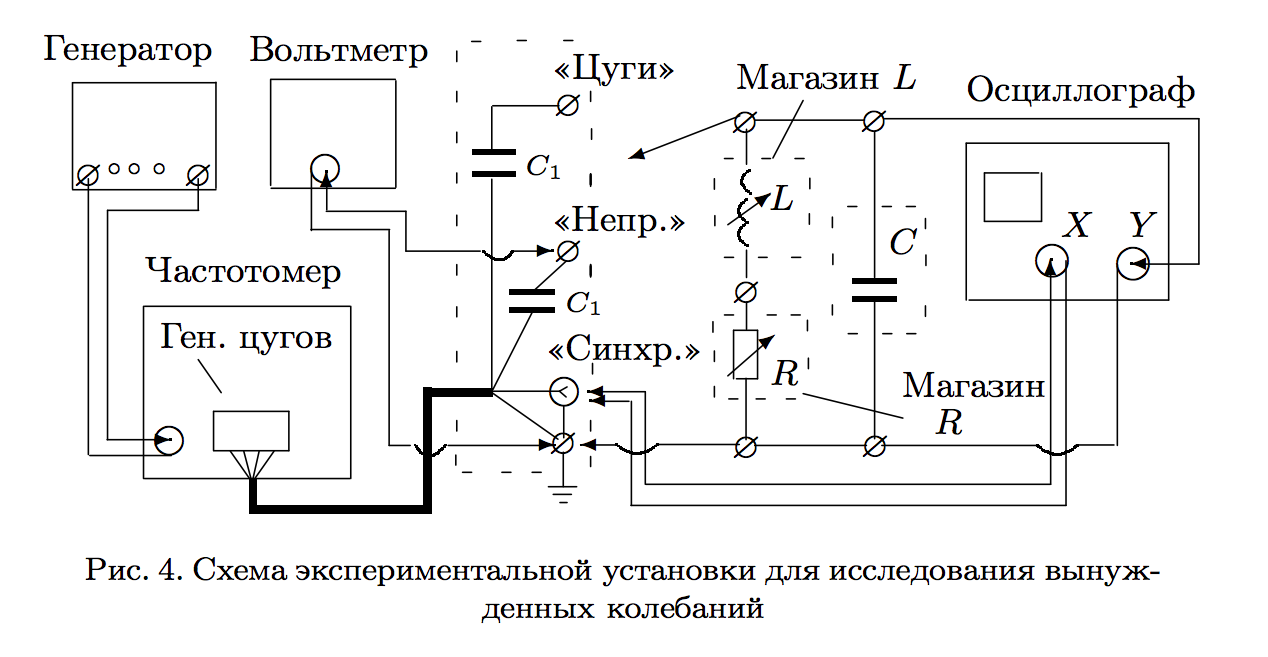
\includegraphics[scale = 0.27]{pic4.png}

\subsection{\label{sec:level2}Задание}

В этом упражнении исследуется зависимость отношения амплитуд
спектральных линий синусоидального сигнала, модулированного низкочастотными гармоническими
колебаниями, от коэффициента модуляции, который определяется с помощью осциллографа.\\
1. Соберите схему, изображённую на рис.~4.\\
2. Подготовьте приборы к работе, следуя техническому описанию (ТО, раздел III, С).\\
3. Изменяя глубину модуляции (ручка 11 на Г6-34), исследуйте зависимость отношения амплитуды боковой линии спектра к амплитуде основной линии ($A_{\text{бок}}/A_{\text{осн}}$) от глубины модуляции $m$ (5–6 значений в диапазоне $0 < m \leqslant 1)$; для расчёта глубины модуляции $m$ по формуле (П.13) измеряйте максимальную $2A_{max}$ и минимальную $2A_{min}$ амплитуды сигнала на экране осциллографа (см. рис. П.6 и П.7).\\
4. При 100\% глубине модуляции ($A_{min}$ = 0) посмотрите, как меняется спектр при увеличении частоты модулирующего сигнала (ручка 10 на Г6-34 поворачивается по часовой стрелке).\\
5. Постройте график отношения $A_{\text{бок}}/A_{\text{осн}}$ в зависимости от $m$. Определите угол наклона графика и сравните с рассчитанным с помощью формулы (П.14).

\section{\label{sec:level1}Обработка измерений.}

\subsection{\label{sec:level2}II}

По измеренной зависимости $\Delta{\nu}(1/\tau)$ построим график и построим невзвешенный метод наименьших квадратов. 

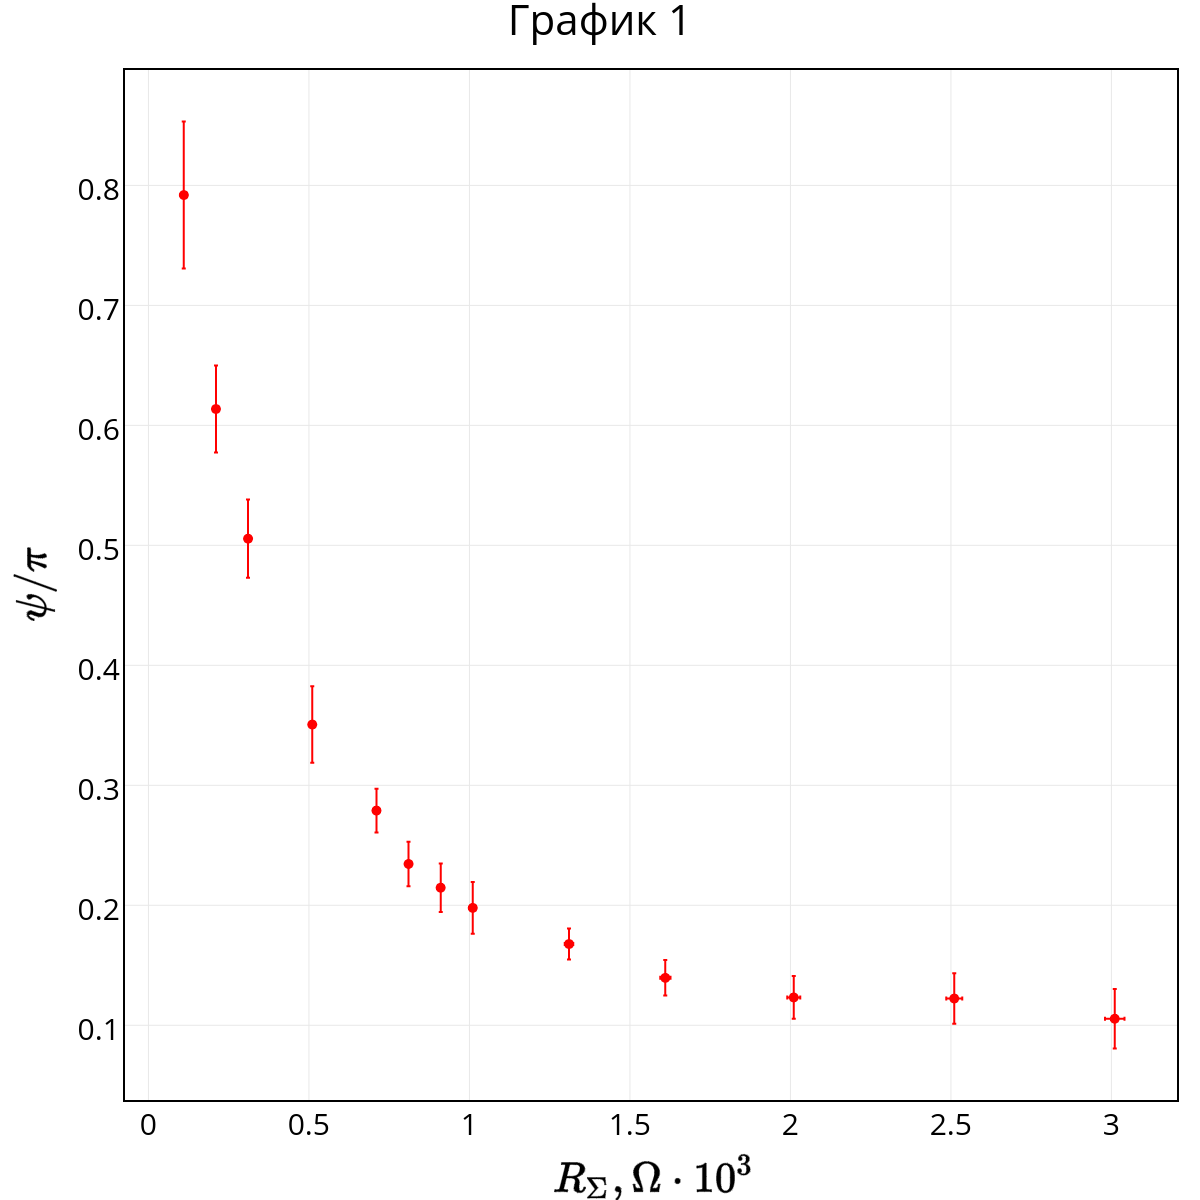
\includegraphics[scale = 0.20]{my_plot1.png}

Результаты построения модели $\Delta{\nu}~=~\alpha~+~\beta(1/\tau)$:
$$ \beta = 1.01 \pm 0.03,~~~~
 \alpha = 0.00 \pm 0.04$$
Что позволяет нам говорить о справедливости соотношения неопределённостей. 

\subsection{\label{sec:level2}III}

По измеренной зависимости $\delta{\nu}(f_\text{повт})$ построим график и аналогично построим невзвешенный метод наименьших квадратов. 

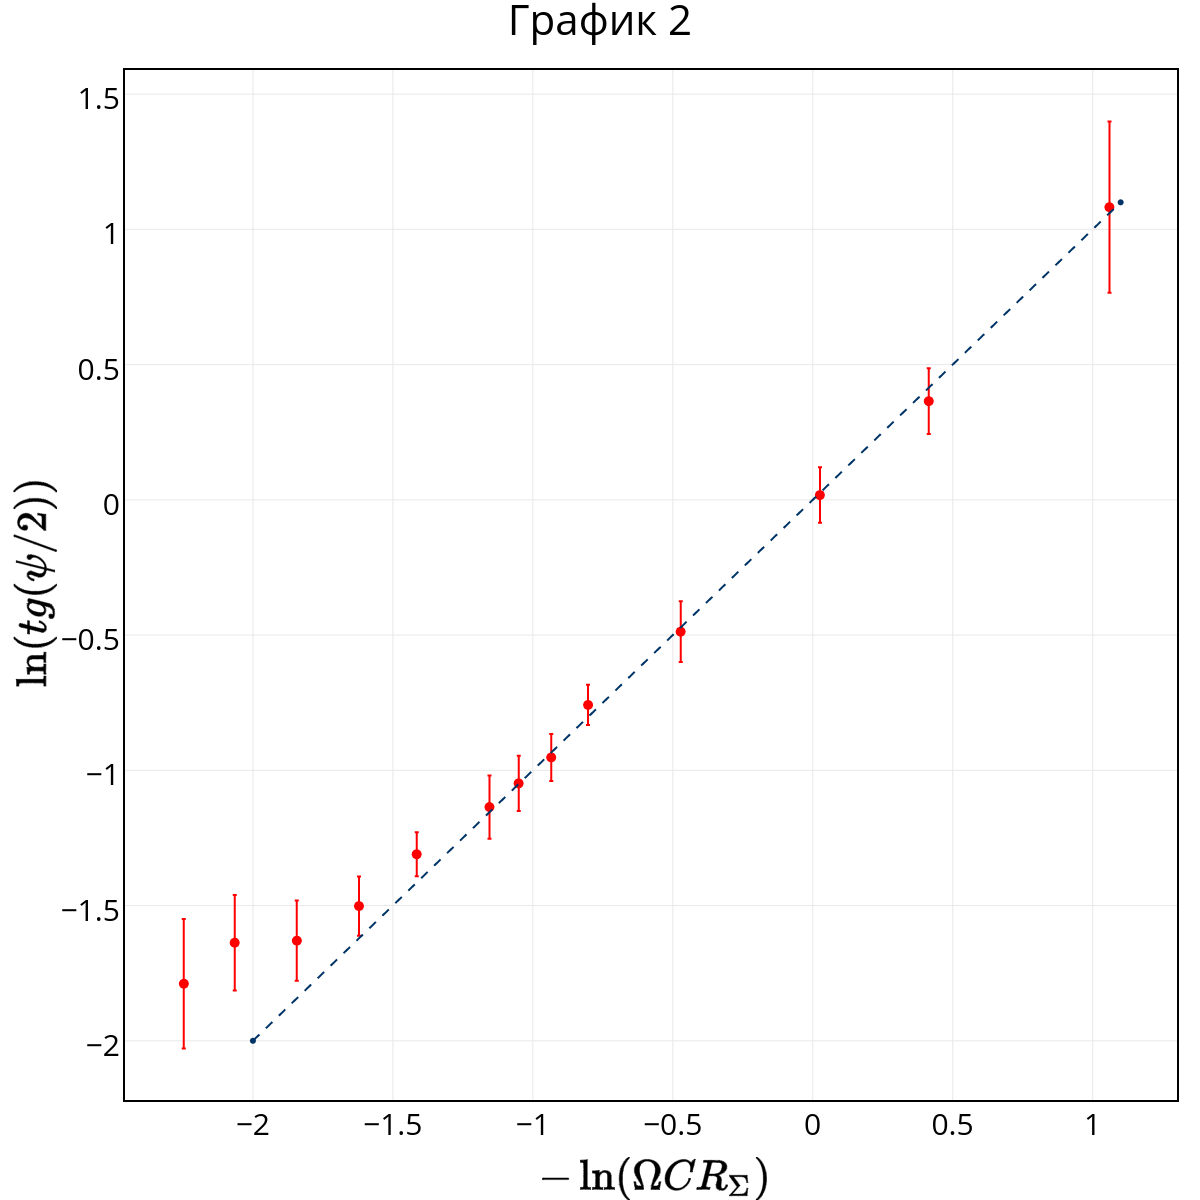
\includegraphics[scale = 0.20]{my_plot2.png}

Результаты построения модели $\delta{\nu}~=~\alpha~+~\beta(f_\text{повт})$:
$$ \beta = 0.99 \pm 0.06,~~~~
 \alpha = 0.00 \pm 0.3$$
Что позволяет нам аналогично говорить о справедливости соотношения неопределённостей. 

\subsection{\label{sec:level2}IV}

Построим график измеренной зависимости отношения амплитуды боковой линии спектра к амплитуде основной линии $(A_\text{бок}/A_\text{осн})$ от глубины модуляции $m$.\\
\\
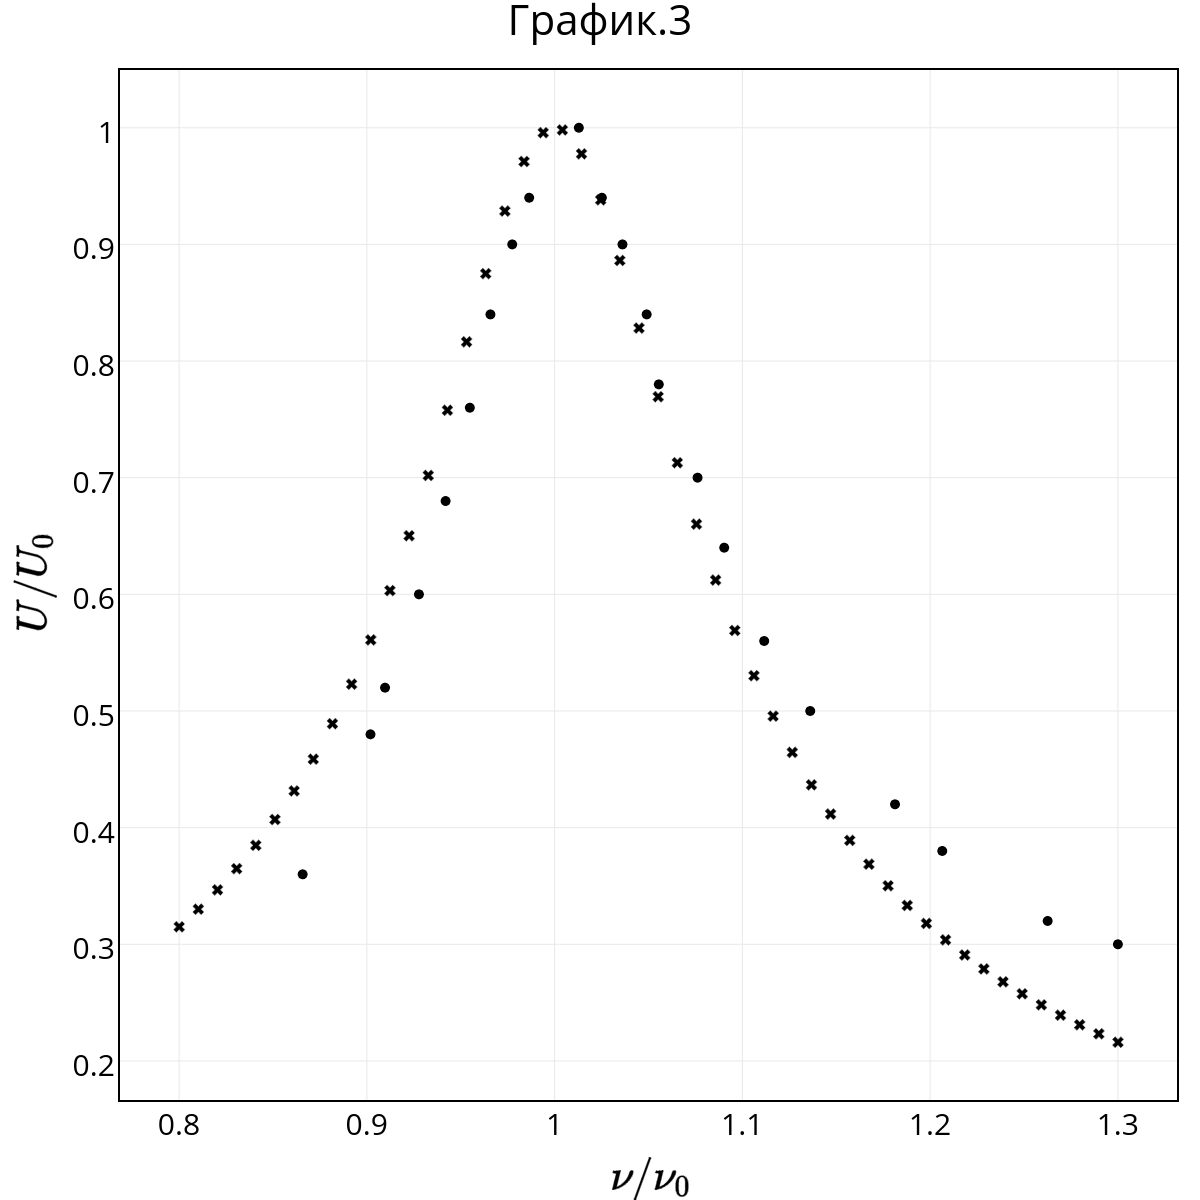
\includegraphics[scale = 0.20]{my_plot3.png}

Построим невзвешенный метод наименьших квадратов и определим угол наклона графика. Стоит напомнить, что согласно теоретической модели значение угла наклона должно быть равным 1/2.

Результат построения:
$$ \beta = 0.54 \pm 0.04,~~~~
 \alpha = 0.00 \pm 0.2$$
 
Предпологаемое значение лежит в 67\% доверительном интервале, на этом уровне значимости можно утверждать совпадение результатов измерения с теорией.

\newpage
\section{\label{sec:level1}Описание спектров.}




\end{document}

